\documentclass{article}

% if you need to pass options to natbib, use, e.g.:
% \PassOptionsToPackage{numbers, compress}{natbib}
% before loading nips_2016
%
% to avoid loading the natbib package, add option nonatbib:
% \usepackage[nonatbib]{nips_2016}

%\usepackage{nips_2016}

% to compile a camera-ready version, add the [final] option, e.g.:
\usepackage[final]{nips_2016}

\usepackage[utf8]{inputenc} % allow utf-8 input
\usepackage[T1]{fontenc}    % use 8-bit T1 fonts
\usepackage{hyperref}       % hyperlinks
\usepackage{url}            % simple URL typesetting
\usepackage{booktabs}       % professional-quality tables
\usepackage{amsfonts}       % blackboard math symbols
\usepackage{nicefrac}       % compact symbols for 1/2, etc.
\usepackage{microtype}      % microtypography

%% Used to style the table
\usepackage{algorithm2e}
\usepackage[usenames,dvipsnames,table]{xcolor}

\usepackage{eqnarray,amsmath}
\usepackage{amssymb}

\usepackage{amsthm}

%\usepackage{subfigure}

\usepackage[pdftex]{graphicx}
\usepackage{caption}
\usepackage{subcaption}

\usepackage{paralist}
\newcommand{\visname}{{\sc MDPv\/is}}
\newcommand{\algname}{MFMCi}
\DeclareMathOperator*{\argmin}{\arg\!\min}

\newtheorem{theorem}{Theorem}
\newtheorem{corollary}{Corollary}

\title{Fast Simulation for Computational Sustainability Sequential Decision Making Problems}

% The \author macro works with any number of authors. There are two
% commands used to separate the names and addresses of multiple
% authors: \And and \AND.
%
% Using \And between authors leaves it to LaTeX to determine where to
% break the lines. Using \AND forces a line break at that point. So,
% if LaTeX puts 3 of 4 authors names on the first line, and the last
% on the second line, try using \AND instead of \And before the third
% author name.

\author{
  Sean McGregor,\textsuperscript{1} Rachel Houtman,\textsuperscript{2} Hailey Buckingham,\textsuperscript{2} \\
  \textbf{Claire Montgomery,\textsuperscript{2} Ronald Metoyer,\textsuperscript{3} and Thomas G.~Dietterich\textsuperscript{1}}\\
  School of Electrical Engineering and Computer Science, Oregon State University\textsuperscript{1}\\
  College of Forestry, Oregon State University\textsuperscript{2}\\
  Department of Computer Science and Engineering, University of Notre Dame\textsuperscript{3}\\
}

\begin{document}
% \nipsfinalcopy is no longer used

\maketitle

\begin{abstract}
  Solving sequential decision making problems in computational sustainability
  often requires simulators of ecology, weather, fire, or other complex phenomena.
  The extreme computational expense of these simulators stymie
  optimization and interactive visualization of decision rules (policies).
  This work presents
  our results in creating an interactive visualization for
  a wildfire management problem whose simulator normally takes
  several hours to run. We successfully generate visualizations
  for a landscape's development over 100 year time spans within
  17 seconds, when the original simulator took several hours.
\end{abstract}

\section{Introduction}

Many computational sustainability problems require making decisions through
time, including invasive species eradication~\cite{Dietterich2013}, and
wildfire management~\cite{Houtman2013}.
Solving these problems involves maximizing expected reward
by finding a policy
that selects the best actions for configurations of the world. For example,
in invasive species problems we perform the ``eradication''
and ``restore'' actions, then receive a reward proportionate to the number
of native and invasive species on the landscape. In the wildfire management domain,
which we use as an example throughout this paper, we select suppression decisions
over 100 year time spans and receive
rewards proportionate to the timber production of the landscape.

In machine learning we formalize
these problems as Markov Decision Processes (MDPs), which
describe the world in terms of a finite set of
states ($S$), a finite set of possible actions that can
be taken in each state ($A$), a function that gives the probability
of entering a state after applying an action in a state ($P$),
and a function providing rewards for taking actions in states ($R(s,a)$).
Since ecological systems typically have more configurations than can be
stored explicitly in a table, the function $P$ is implemented
as a simulator that generates hypothetical futures (trajectories)
subject to a policy.
These simulators are often sufficiently expensive to run that
we must find ways to minimize their use when optimizing policies.

Many algorithms economize simulator expense by constructing
trajectories for a policy based on the pre-computed results of a different policy.
This \emph{off-policy} policy evaluation is particularly important
for supporting interactive visualization \cite{McGregor2015a}, which
allow ecologists, land managers, developers, and policy makers
to validate the assumptions incorporated into simulators.

Fonteneau et al.'s \cite{Fonteneau2010c}'s Model Free Monte Carlo (MFMC) method
is one approach for off-policy policy evaluation.
MFMC synthesizes trajectories by piecewise \emph{stitching} state transitions
together from a database of
previously-simulated state transitions.
Since MFMC replaces simulations with a series of database queries, it
can generate trajectories without waiting for
the simulator to run.

Our work currently under review for the 2016 conference on Neural Information Processing Systems (NIPS)
addresses two ``curses of dimensionality'' that make MFMC impractical for
large state space MDPs that are typical of computational sustainability problems.
First, it is difficult to sample sufficient state transitions to gain database coverage
of high dimensional state-action spaces \cite{Hallak2015}. Second, it is difficult
to determine similarity among state-action samples in higher dimensions.
We solve these curses of dimensionality with a new algorithm, \algname,
for problems with exogenous state variables,
such as weather in a wildfire management problem.

Since our goal is to support interactive MDP visualization, we use visual properties
of the MDP visualization \visname{} \cite{McGregor2015a} to evaluate the performance of \algname.
We use the unitless measurement of ``visual fidelity error,'' which is a measure of
how similar \visname{} looks under \algname\ when compared to the visualization generated
from the ground truth simulator.

We demonstrate \algname\ on a computationally expensive wildfire, timber,
vegetation, and weather simulator that takes hours to generate single
trajectories. The aim of the wildfire management simulator is to inform
wildfire suppression policies that determine whether the US government
will suppress a wildfire.

The fire simulator spreads fire spatially from an ignition point
according to the surrounding pixel layers and the hourly weather
sampled from 26 historical weather years.
Weather variables include hourly wind speed,
wind direction, cloud cover, minimum temperature, maximum temperature,
temperature, humidity, and precipitation.
We use \algname\ to synthesize trajectories
by modeling the weather time series and ignition locations as exogenous variables.
The weather is exogenous because, to a first approximation,
neither the actions not the landscape influence the weather.
Ignition location is exogenous to the landscape because tree cover does not affect
the ignition's spatial probability
distribution. Additionally, timber harvest and vegetation growth are deterministic
functions of the landscape, which means every state transition contains their results.

In the next section we provide additional theoretical background on our
algorithm leveraging independencies of exogenous state variables.
In the results section we describe its performance in terms of our
computationally expensive wildfire management problem domain.

\section{Methods}

We address MFMC's dimensionality issue by exploiting \emph{transition independencies}
that factor the state space into \emph{Markovian} variables that transfer between time steps,
and \emph{exogenous} variables that are combined with the Markovian variables at every time step.
For example, in the wildfire domain, the state of the trees from one time step to another
is Markovian, but we make decisions in response to exogenous weather events such as rain, wind, and lightning.
By factoring out exogenous variables, we can synthesize trajectories
from the (lower dimensional) Markovian state space.

We can define the transition independencies in terms of
probabilistic graphical models in Figure \ref{fig:PGMMDP}.
The standard MDP transition is in Figure \ref{fig:MDP1}. Figure \ref{fig:MDP2} shows
the setting of prior work \cite{Fonteneau2010c,Hallak2015}
that model ``unobservable random disturbances'' ($w_u$).
We call these \emph{unobservable exogenous variables},
which are distinct from the \emph{observable} exogenous variables
($w_o$ in Figure \ref{fig:MDP3})
of interest in this work.

MFMC normally selects state transitions from a database by
matching a state action pair $(s,a)$
to the first two elements $(s',a')$ in the 4-tuple
$(s',a',r',s_{result})$.
It then adopts $r'$ as the one step reward and $s_{result}$
as the resulting state. In our approach, we show how to
decompose $s$ into $(x,w_o)$ and then only match $x$ against $x'$
in the 5-tuple $(x',w_{o}',a',r',x_{result})$.
Our algorithm, \algname, then adopts $w_{o}'$ as the instance of
the exogenous random variable, $r'$ as the reward, and $x_{result}$
as the resulting state. In order for this to work correctly,
two conditions must hold. First, the values of $w_o$ in each state must be
independent and identically distributed.
Second, the database must contain a separate tuple
$(x',w_{o}',a,r',x_{result})$ for each possible action $a$ (we refer to sets of tuples containing
the same $x$ and $w$, but different $a$ as \emph{transition sets}) so
that we can look up the action 
corresponding to both the $x$ and $w_o$.
Since we guarantee an action consistent with the policy will be in the nearest
tuple, we can reduce the dimensionality
of the search for the nearest tuple to a distance in the space of $x$ from the $(s,a)$ space.

\begin{figure}
    \centering
    \begin{subfigure}[t]{0.30\textwidth}
        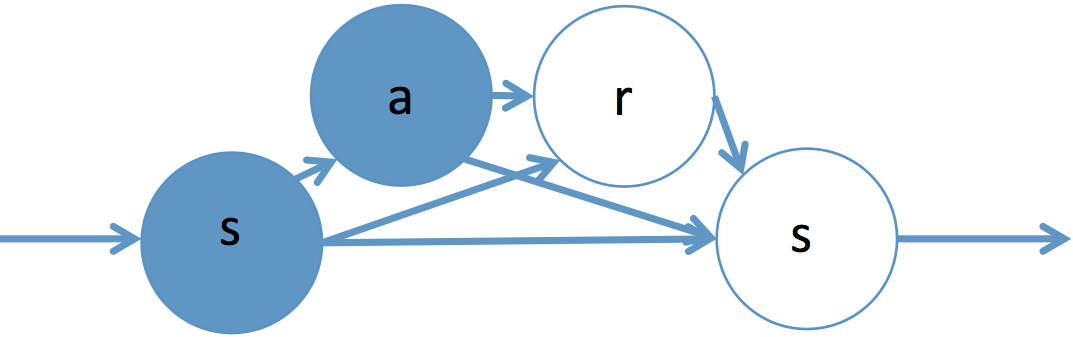
\includegraphics[width=\textwidth]{png/mdp1ras.png}
        \caption{The standard MDP transition.}
        \label{fig:MDP1}
    \end{subfigure}
    ~~~
    \begin{subfigure}[t]{0.30\textwidth}
        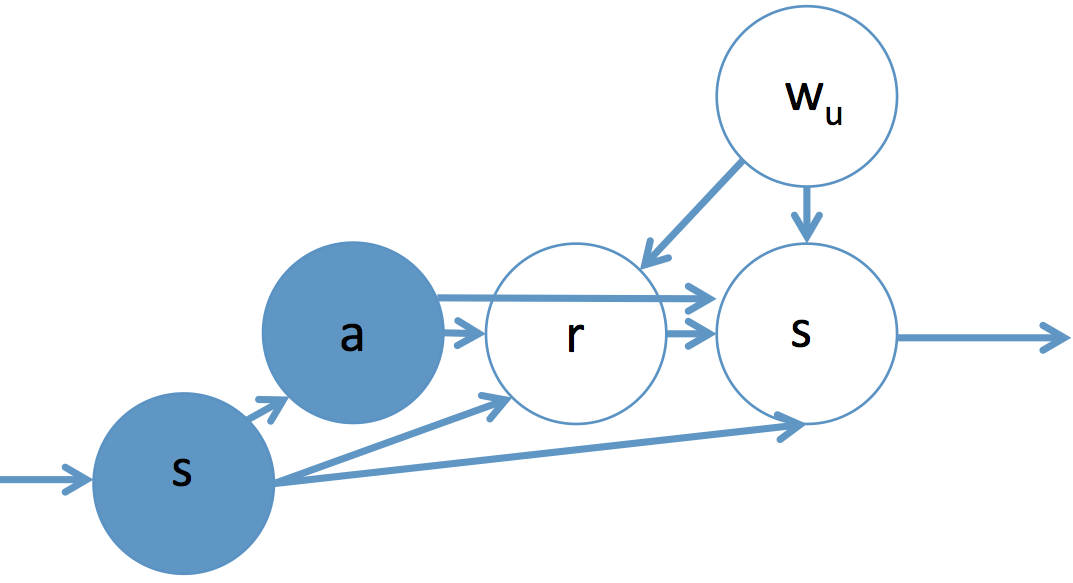
\includegraphics[width=\textwidth]{png/mdp2ras.png}
        \caption{
        MDP transition with unobservable exogenous variables ($w_u$).
        }
        \label{fig:MDP2}
    \end{subfigure}
    ~~~
    \begin{subfigure}[t]{0.30\textwidth}
        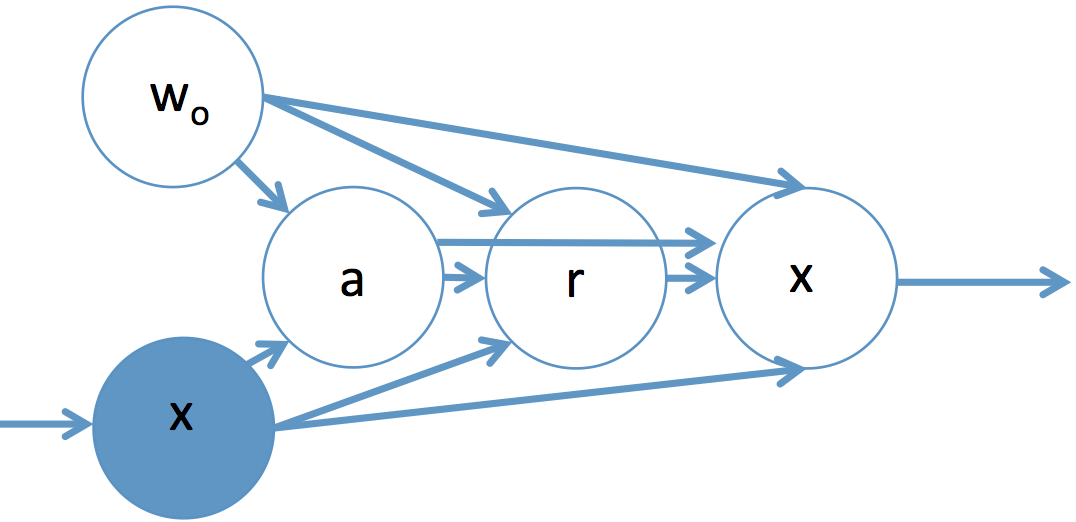
\includegraphics[width=\textwidth]{png/mdp3ras.png}
        \caption{
        MDP transition with \emph{observable exogenous} variables ($w_o$).}
        \label{fig:MDP3}
    \end{subfigure}
    \caption{MDP probabilistic graphical models.}
    \label{fig:PGMMDP}
\end{figure}

Fonteneau et al.~\cite{Fonteneau2010c} adopt Lipschitz continuity assumptions on the
transition, reward, and policy functions to prove bounds on the
bias and variance of the estimated return of a policy. Their bounds depend on
the Lipschitz constants, the number of generated trajectories,
and the sparsity of the database of transitions.
We employed a similar set of assumptions,
but by reducing the dimensionality of the database's space,
we tighten the bounds derived from these assumptions.

\section{Results and Discussion}

We define policies in terms of two thresholds: $\pi_E$ and $\pi_{ERC}$.
Policy $\pi_E$ is the maximum time until end of fire season at which
the fire will be allowed to burn.
$\pi_{ERC}$ is the Energy Release Component (ERC) at which the
fire is suppressed.
We seek to visualize trajectories for
all combinations of $\pi_E$ and $\pi_{ERC}$.

\begin{figure}
    \centering
    \begin{subfigure}[b]{0.49\textwidth}
        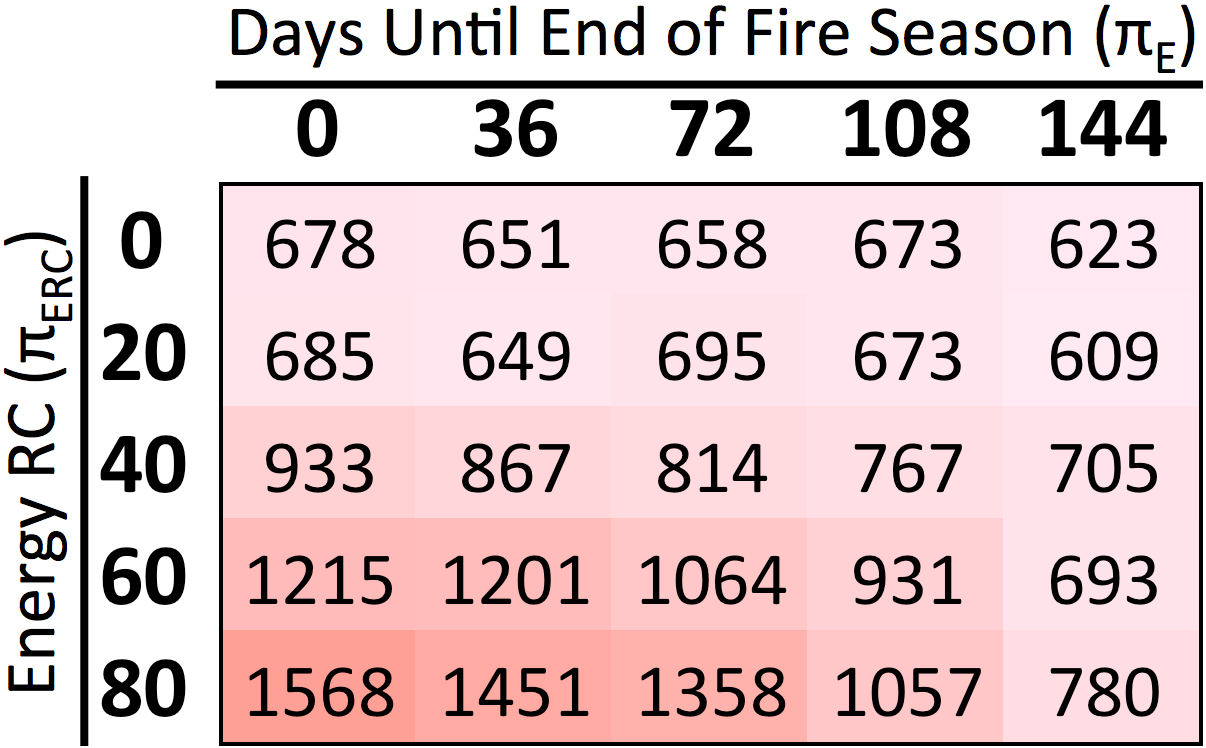
\includegraphics[width=.88\textwidth]{png/heatmap2.png}
        \caption{
          Visual fidelity error in weighted pixels
          across the policy space for the factored metric.
          The darkness of the cell is proportionate to the number of unsuppressed
          fires for the policy.
          }
        \label{fig:factored-fidelity}
    \end{subfigure}
    ~ %add desired spacing between images, e. g. ~, \quad, \qquad, \hfill etc. 
      %(or a blank line to force the subfigure onto a new line)
    \begin{subtable}[b]{0.49\textwidth}
        \centering
        \begin{tabular}{llll}
          \toprule
          Database Size & Policy & $\mu$ & $\sigma$ \\
          \midrule
          $|d|$ & $\Pi_{(ERC,E)}$ & 880 & 281 \\
          Unbiased $\frac{1}{2}|d|$  & $\Pi_{(ERC,E)}$ & 913 & 273  \\
          Biased $\frac{1}{2}|d|$ & $\Pi_{(ERC,E)}$ & 554 & 113 \\
          $|d|$ & $\Pi_{L}$ & 750 & 172 \\
          Unbiased $\frac{1}{2}|d|$ & $\Pi_{L}$ &  894 &  4 \\
          Biased $\frac{1}{2}|d|$ & $\Pi_{L}$ &  1,224 &  20  \\
          \bottomrule
        \end{tabular}
        \caption{
        Visual fidelity error under the full, half (unbiased and biased) databases.
        The policy class $\Pi_{(ERC,E)}$ matches the policies of
        Figure \ref{fig:factored-fidelity}.
        The policy class $\Pi_{L}$ has two ignition location-based policies.
        }
        \label{tab:debiased}
    \end{subtable}
\end{figure}

Our quantitative evaluation showed several interesting results. First,
Figure \ref{fig:factored-fidelity} shows our factored metric performs well
across the entire policy space. The relatively higher values in the lower
left of the chart result from leaving most of the sample's wildfires unsuppressed. Since
unsuppressed fires have greater variance in the number of burned
crown pixels (tree foliage) and surface pixels,
it would take more samples to drive down
the Monte Carlo variance of the visualization than is practical.

Table \ref{tab:debiased} lists visual fidelity error for two policy classes using
both the full database, and a database with half as many samples.
We constructed the halved databases
by either removing all but one transition from the transition sets (biased),
or by removing all samples associated with even-numbered
trajectories in the database (unbiased). The additional policy class $\Pi_{L}$
suppresses all fires on one half of the landscape and otherwise
allows them to burn.
The results show the transition set is more valuable
for synthesizing trajectories for policy classes not found in the transition database.
Such novel policies are an important part of exploratory analysis that
will be performed by foresters.

\algname\ generates trajectories more than 1200 times faster
than invoking the simulator.
Without these speedups, interactive visualization and
policy exploration of wildfire policies is not possible.

\small

\bibliographystyle{abbrv}
\bibliography{references}

\end{document}
